% ----------------------------------------------------------------------------------------
% Name: Related Work and Basic Principles
% Author: Emmanuel SCHWARTZ
% Date: November 2016
% Description: Related Work and Basic Principles Chapter for my master thesis paper
% ----------------------------------------------------------------------------------------
\section{Related Work}


\subsection{Towards Cloud-Based Decentralized Storage for IoT}
\subsection{Prototype of cloud based document management for scientific work validation}
\subsection{Sia}

\section{Basic Principles}

\subsection{Reminders in Cryptography: Hash, Signature and Merkle tree}
\subsubsection{Hash Function}
\paragraph{}
A hash function is an algorithm that generates a numeric, or fixed-size character output from a variable-sized piece of text or other data (Figure 2.1). An essential property is that it is practically impossible to reverse it: the hash of a datum by the function is calculated very efficiently, but the inverse calculation of an input hash to find a datum is infeasible. For this reason, such a function is said to be one-way.The input data is often called the message, and the output (the hash value or hash) is often called the message digest or simply the digest.

\paragraph{}
{\setlength{\parindent}{0cm}
An ideal cryptographic hash function has the following four properties:
}

\begin{itemize}
  \setlength\itemsep{0em}

  \item Collision resistant: It is hard to find for a given \emph{m1} any \emph{m2} with \emph{H(m1) = H(m2)}. Two messages can't have the same footprint.
  \item Non-reversible: It is hard to find \emph{m} given \emph{H(m)}. It is impossible for a given hash value to construct a message having that hash value except by trying all possible messages.
  \item Fast: The hash value of a message is calculated very quickly
  \item Unique: A small change to a message should change the hash value so extensively that the new hash value appears uncorrelated with the old hash value.

\end{itemize}

\paragraph{}
The most common hash functions are listed below:
\begin{itemize}
  \setlength\itemsep{0em}

  \item MD4 and MD5 (Message Digest) were developed by Ron Rivest. MD5 produces 128-bit hashes by working the original data in blocks of 512 bits.
  \item SHA-1 (Secure Hash Algorithm 1), like MD5, is based on MD4. It also operates from blocks of 512 bits of data and produces condensed bits of 160 bits at the output. It therefore requires more resources than MD5.[*]
   \item SHA-2 (Secure Hash Algorithm 2) has been published recently and is intended to replace SHA-1. The main differences are in the possible chopping sizes: 256, 384, or 512 bits. It will soon be the new reference in terms of hash function.[*]
  \item RIPEMD-160 (Ripe Message Digest) is the latest version of the RIPEMD algorithm. The previous version produced 128-bit digits but presented significant security flaws. The current version remains safe for now; It produces as the name indicates the condensed 160 bits. A final point concerning it is its relative greediness in terms of resources and in comparison with SHA-1 which is its main rival.
\end{itemize}

\paragraph{}
\begin{figure}[!h]
\begin{center}
\resizebox{\columnwidth}{!}{%
\begin{tabular}{|c|c|}
\hline
	text & hash(text)\\
\hline
	Here is a long text & faf3d315060c6b887e826e7a65992539e846233cea3f2e4cde4d9351b4f00193\\
\hline
	Hello World! & 7f83b1657ff1fc53b92dc18148a1d65dfc2d4b1fa3d677284addd200126d9069\\
\hline
	Hello World. & f4bb1975bf1f81f76ce824f7536c1e101a8060a632a52289d530a6f600d52c92\\
\hline
	Hello World. & f4bb1975bf1f81f76ce824f7536c1e101a8060a632a52289d530a6f600d52c92\\
\hline
\end{tabular}%
}
\caption{Example of an hash function}
\end{center}
\end{figure}

\subsubsection{Signature}

The digital signature[*] is a mechanism to guarantee the integrity of an electronic document and to authenticate the author by analogy with the handwritten signature of a paper document. It must allow the reader of a document to identify the person or organization that has affixed his/her signature. Moreover, a digital signature mechanism must have the following properties:

\begin{itemize}
  \setlength\itemsep{0em}

  \item Authentic: the identity of the signatory must be able to be found with certainty
  \item Forgery: the signature can not be falsified. Someone can not pretend to be another
  \item Not reusable: the signature is not reusable. It is part of the signed document and can not be moved to another document.
  \item Unalterable: A signed document is unalterable. Once it is signed, you can not change it
  \item Irrevocable: the person who signed can not deny it

\end{itemize}

In order to sign a document, the common way to do it is to use keys. Each user has a pairs of keys: a public one, called PubKey, and a private key, nammed PrivKey.
\begin{figure}[htp]
\centering
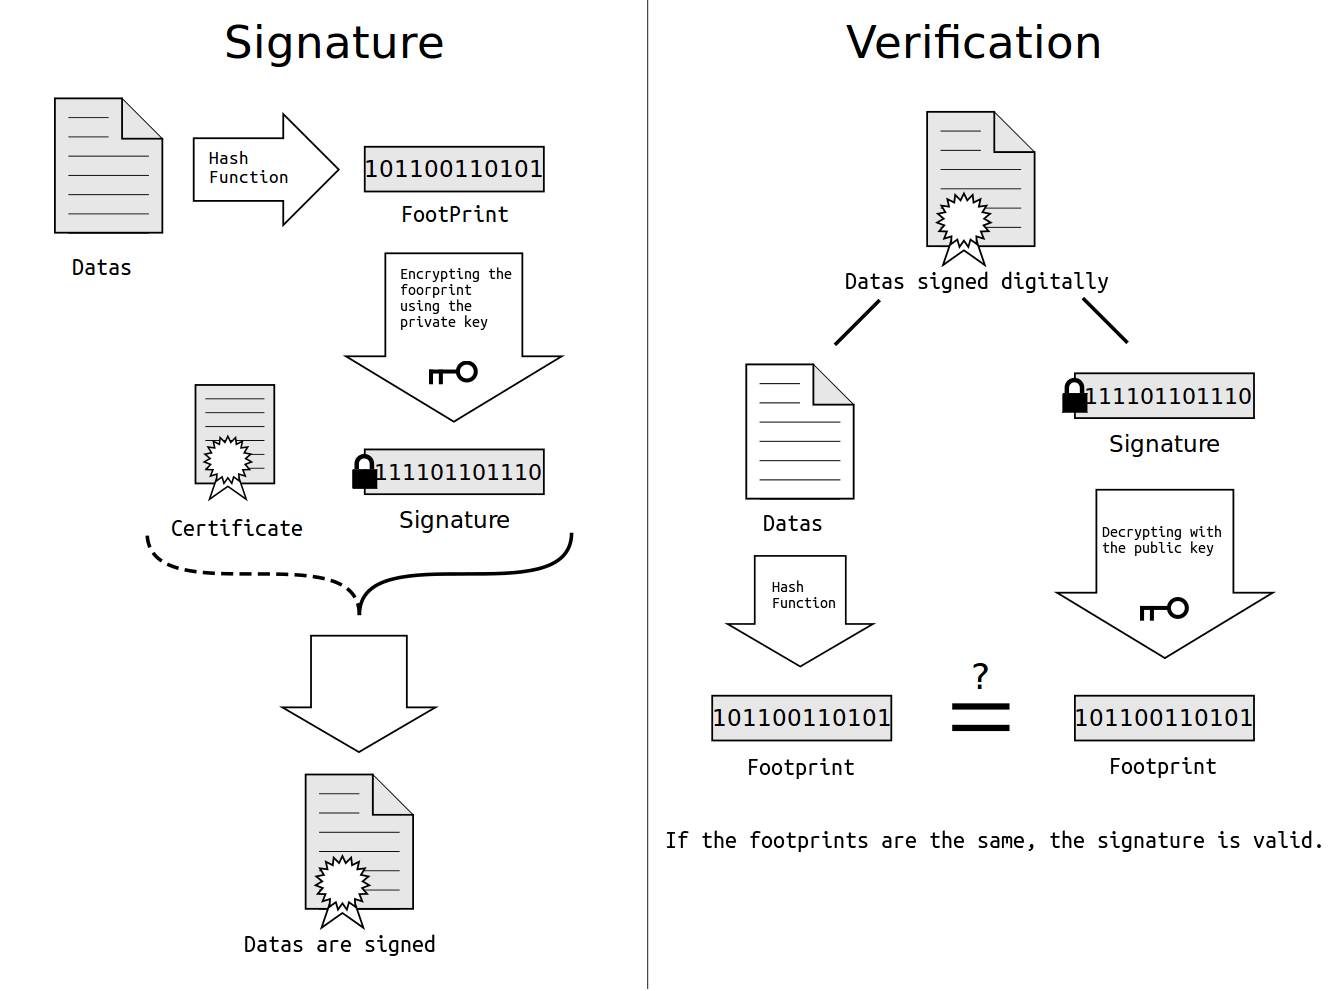
\includegraphics[scale=0.30]{/home/emmanuel/Documents/masterThesis/doc/ressources/signature.png}
\caption{Digital signature diagram}
\label{}
\end{figure}

\subsubsection{Merkle Tree}
\paragraph{}
Created in 1979 by Ralf Merkle, one of the pionner of the asymetrical cryptography, the Merkle tree, or hash tree, is data structure containing an information summary of a data volume, which are usually big. (see figure X.X).
\begin{figure}[h!]
\centering
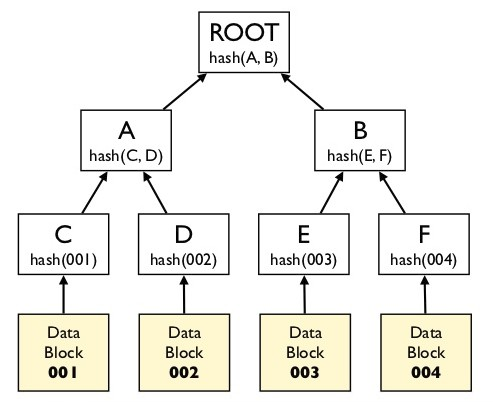
\includegraphics[scale=0.50]{/home/emmanuel/Documents/masterThesis/doc/ressources/merkle.png}
\caption{Merkel tree}
\label{}
\end{figure}
\paragraph{}
The principle of a hash tree consists of decomposing the input data into a set of blocks of identical size. These blocks are the leaves of the tree. They are usually completed with neutral values, such as zeros, so as to obtain blocks of the desired size. The higher level nodes are then obtained by compressing the nodes of the current level using a hash / compression function until only one node is obtained: the Merkle root hash.
With this principle, the hash tree gives a unique footprint of all data. By just storing the root hash, it is very easy to large data comparaison by anylysing only the Merkle root hashes without the need to download these large data files. Moreover, it also can detect if a data has been modified. 
\paragraph{}
The field of applications of the Merkle tree are wide-spreaded going from Peer-2-Peer[*] networks to GIT[*] or even ZFS file system[*]

\subsection{Blockchains}
\paragraph{}
This section will explain blockchains and its components in details through the famous cryptocurrency: Bitcoin.

\subsubsection{What is a blockchain?}
\paragraph{}
Bitcoin brought with him a new concept: The system operates without central authority or single administrator, but in a decentralized way thanks to the consensus of all the nodes of the network, this means everynode have to reach an agreement in order to go to the next step. 
\paragraph{}
A blockchain is a public ledger of all transactions that have ever been executed. Based on a distributed database, it maintains a continuously-growing list of a ‘completed’ blocks are added to it with a new set of recordings. As its name suggests, the blockchain is a succession of blocks. The blocks are added to the blockchain in a linear and chronological order. Each blocks are linked by incorporating the hash of the previous block, showed in Figure 2.3:
\begin{figure}[htp]
\centering
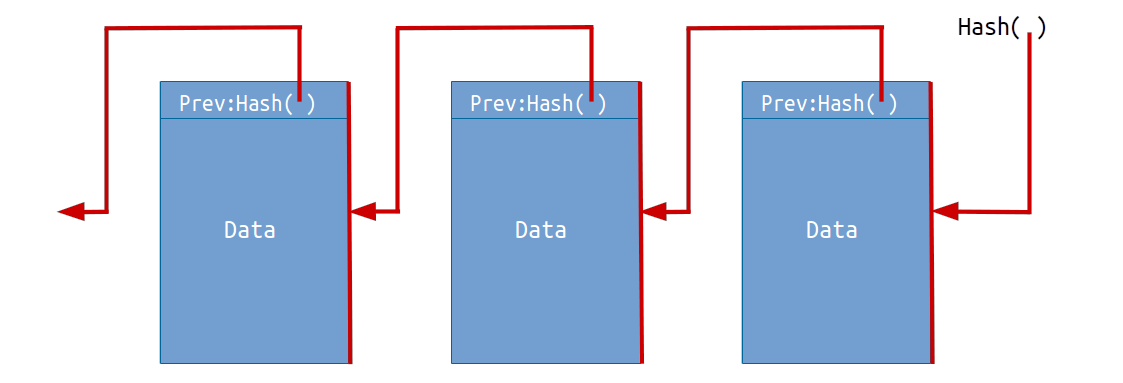
\includegraphics[scale=0.42]{/home/emmanuel/Documents/masterThesis/doc/ressources/blockchain_block.png}
\caption{Global structure of a blockchain}
\label{}
\end{figure}
\newline
With this structure, blockchains are inherently resistant to modification of the data: Once recorded, the data in a block cannot be altered retroactively. Moreover, since it is working in a decentralized way, each node (e.g computer connected to the network) has and need to have a copy of all transactions. Therefore, it is easy to verify a transaction easily with this record since they are public.

\subsubsection{Transactions}
A transaction is the record of transfering money from a person A to a person B, following these two easy but essential rules: 
\begin{itemize}
  \setlength\itemsep{0em}

  \item It is only possible to transfer coins that we owned, using transaction "Pay"
  \item It is only miners that can create bitcoin, using a transaction "Coinbase"
\end{itemize}


-problem \#1: give coin at the same time 
\newline
-problem \#2: How can we split a coin 
\newline
-problem \#3: problem of the double spent 
- propagation of a transaction to all the nodes
\newline
\subsubsection{Block}
- detail of a block
\newline
- example of a block
\newline
- pseudo code of what are all the steps to confirm one block
\newline
- Fork
\newline
- How can be the the transaction is valid
\newline
- transaction every 10 mins
\newline
-how much transaction per block
\subsubsection{Miners \& Proof of Work}

\subsubsection{Nounce}
- complexity varies
\newline
- calculation of hashes
\newline 
- random hash
\newline
- pseudo code how to resolve a hash
\newline
- example of a nounce
\subsubsection{Payment}
- Evolution of the difficulty
\newline
- problem of pool mining
\subsection{Ethereum: the 2.0 blockchain}
\subsubsection{What is Ethereum?}
- blockchain 2.0
\newline
- blockchain that can store 
\newline
- faster blockchain but engender new problems
\newline
- really expensive to store data
\newline
- everything is public
\subsubsection{GHOST}
- orphan blocks
- godfather blocks
- scheme
 \subsubsection{Accounts}
 - ID
 \newline
 - balance
 \newline
 - storage root
 \newline
 - code hash
 \newline
 - one account per user / smart contract
 \newline
 - storage : non accessible outside account
 \newline
 \begin{figure}[htp]
\centering
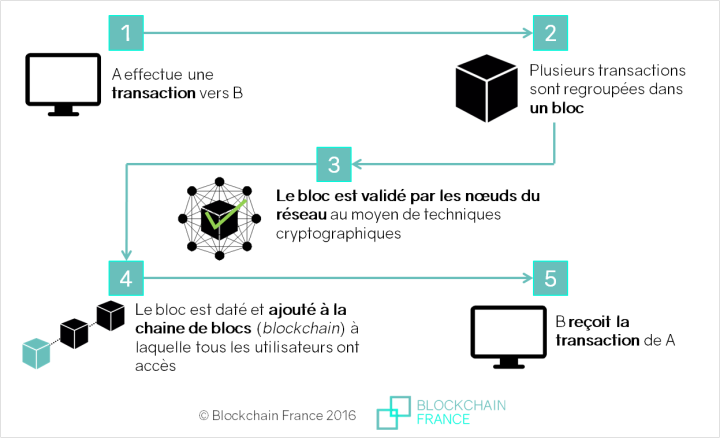
\includegraphics[scale=1.00]{/home/emmanuel/Documents/masterThesis/doc/ressources/blockchain_summary.png}
\caption{Blockchain secure workflow}
\label{}
\end{figure}
 1 	Digitally signed transaction initiation
2 	Transaction is sent to miner who verifies transaction
3 	Transaction is broadcast to all connected nodes as block
4 	Network accepts transaction if data is valid
5 	Receiver receives the transaction
  \subsubsection{Smart Contracts}
- stored in blockchain
\newline
- can modify the state of the blokchain
\newline
- associted to one unique account
\newline
- conditions/ loops / unlimited stacks \& memory/
\newline
- example of transaction with ethereum
\newline
- smart contract call talk to other smart contracts  
\newline
- properties 
- constrainsts
\newline
- solidity, serpent, LLL
\newline
- Dapps
\subsubsection{Oracle}
- smart contracts that can provide pieces of information of the external world
\newline
- synchrone mode
\newline
- asynchrone mode
\newline
\textbf{WHY DO WE DO THIS ?}

\subsubsection{differences with bitcoin}
blockchain state machine with transaction which modify the state
\subsection{Decentralized Storage Providers}

\subsubsection{IPFS}

\subsubsection{StorJ}

\subsubsection{Dat-data}

\subsubsection{Swarm}

\subsubsection{Overall Requirements Examination}

\subsection{Access control????}

